% !TEX root=./proposal.tex

\subsection{研究背景和科学意义}


%0.人工智能技术很广泛,智能软件越来越多进入人们的生活1.于此同时,其安全问题也得
%到越来越多的关注2.当前的研究主要针对单个智能组件研究其脆弱性,如对抗攻击,后门
%攻击等。近年来,逐渐有少量研究深度学习基础包和依赖库的漏洞,然而如何利用第三方
%开源组件漏洞去激活智能组件的脆弱性研究较少。
%举例
%挑战:3点
%本项目的研究意义3点

%
% 0.人工智能技术很广泛,智能软件越来越多进入人们的生活
近年来,在数据和算力的驱动下,人工智能技术取得了巨大成功,已在世界范围内引领了一
轮新的产业革命,是国际数字规则博弈的重要领域之一。人工智能技术对复杂问题的解决能
力使其研究成果逐渐从实验室走向实际应用,如人脸识别~\cite{meng2021magface}、自动
驾驶~\cite{zhang2018deeproad}、机器翻译~\cite{johnson2017google}、智慧医疗
~\cite{zhang2021tau}等领域。智能软件(Intelligence Software)是指\textbf{{采用人
工智能技术来演绎、推理和解决问题的软件系统}}。Gartner预测,2022年全球智能软件收
入总额将达到625亿美元,相比2022年增长
21.3\%\footnote{https://www.gartner.com/cn/newsroom/press-releases/20211207-ai-software-forecast}。
为了提高开发效率,智能软件的构建过程通常使用大量第三方开源组件为基础,智能软件由
\textbf{嵌入的人工智能组件、基础框架组件以及其它第三方组件}等多类型组件共同组成
(见\cref{fig:ch1:aisoftware})。其中,人工智能组件指以神经网络模型为代表的智能
模型,例如循环神经网络、卷积神经网络等。基础框架组件是指用来构建智能组件的基础依
赖库,常用的框架有PyTorch、Tensorflow、Caffee2等。除此以外,作为一类特殊的软件系
统,智能软件还可能使用大数据处理、包装器与压缩、统计分析、数据预处理等第三方组
件。

%美国白宫颁布了《维护美国在人工智能领域领导地位》、《国家人工智能研发战略》;欧
%盟致力于打造“从实验室进入市场”,发布《2021人工智能协调计划审查》;俄罗斯发布
%《2030年前国家人工智能发展战略》; 2017年7月,我国国务院印发《新一代人工智能发
%展规划》,旨在构筑我国人工智能发展的先发优势,2019年科技部印发《国家新一代人工
%智能创新发展试验区建设工作指引》,全面提升人工智能创新能力和水平。
\begin{figure}[htp]
    \centering
    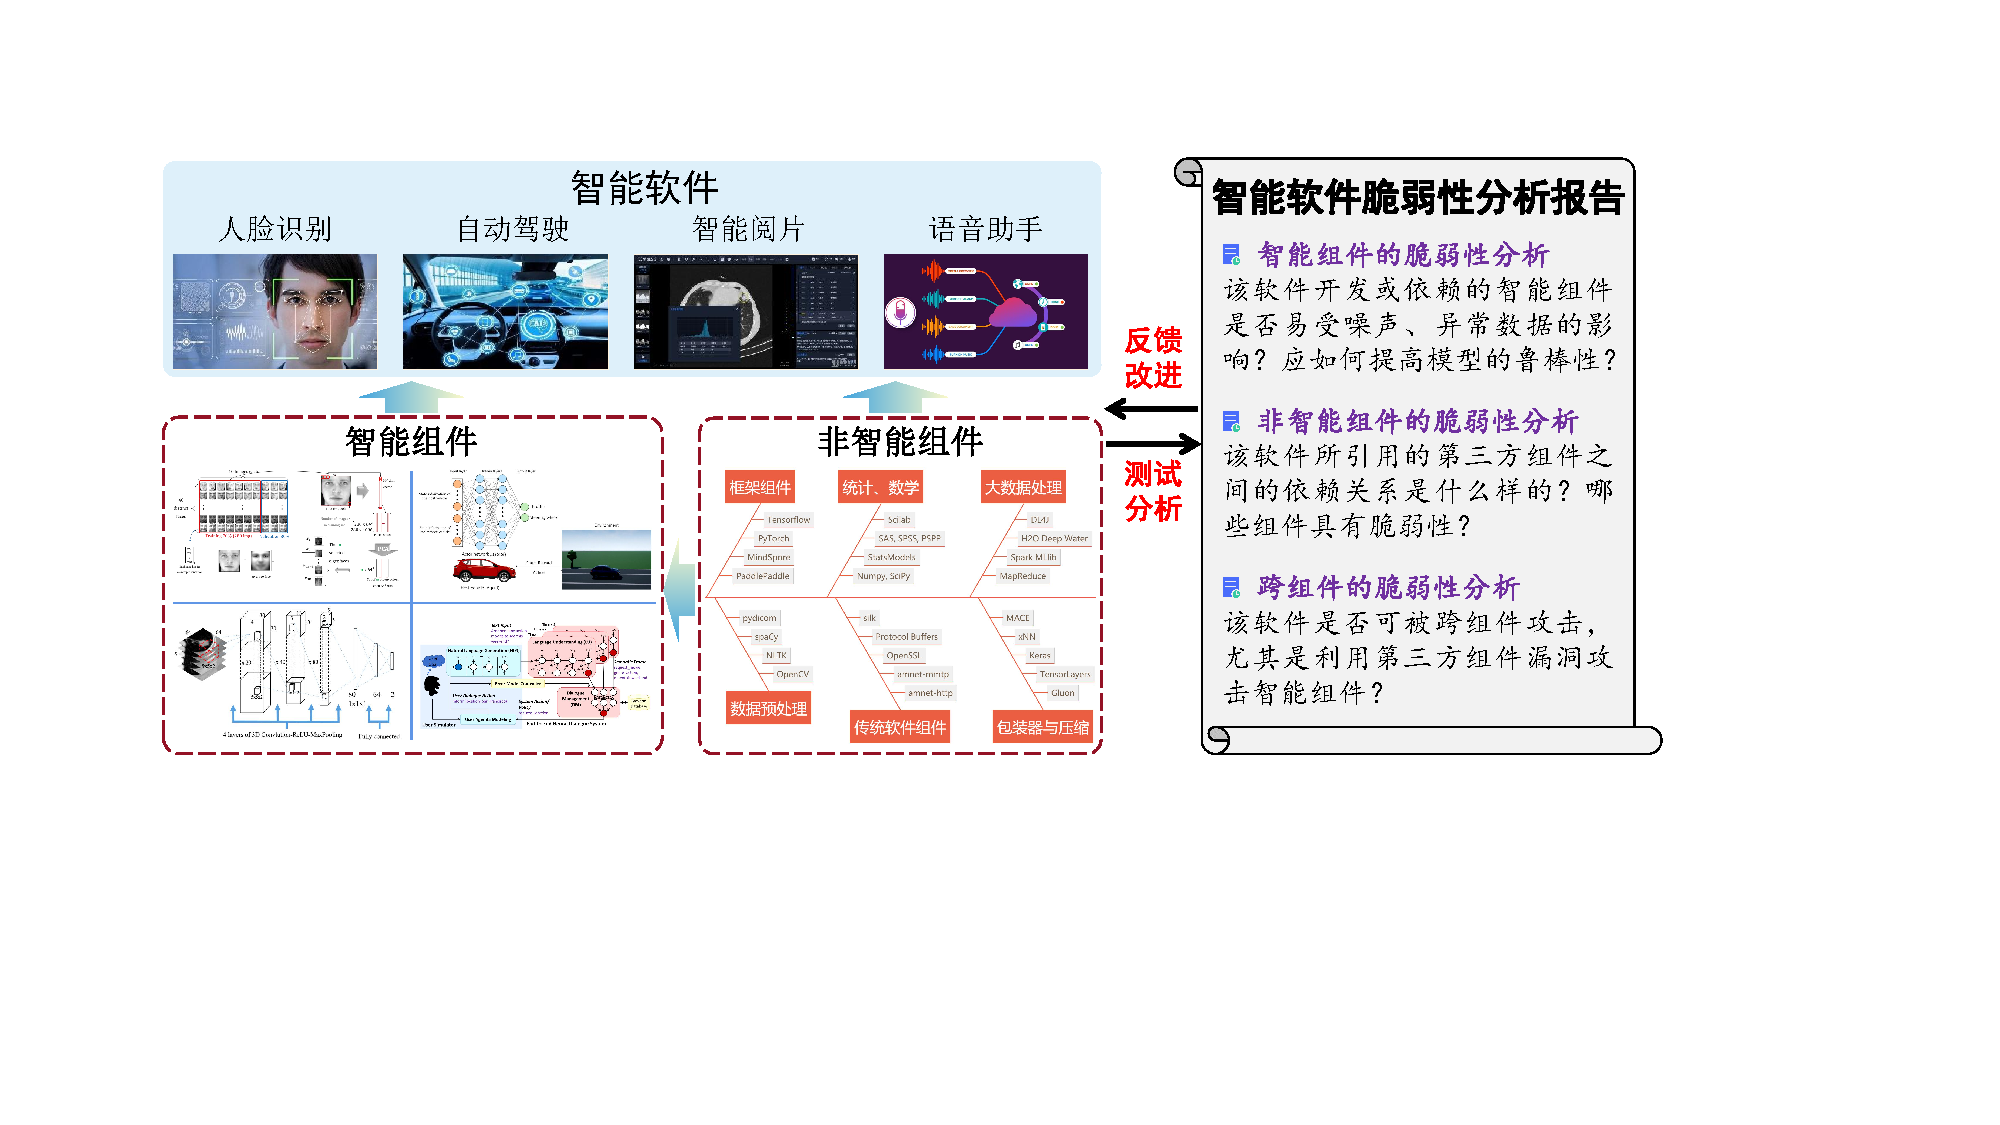
\includegraphics[width=0.98\linewidth]{ch1_AIsoftware.pdf}
    \caption{智能软件依赖于多类型组件,XXX}
    \label{fig:ch1:aisoftware}
\end{figure}


虽然人工智能技术已获得巨大成功,但\textbf{一个可靠的、安全的智能软件系统是其在关
键领域上成功落地的前提}。2018年3月,一辆处在自动驾驶状态的Uber撞击一名女子,致其
不幸身亡,同年7月,Uber宣布停止研发自动驾驶货车。Szegedy等人首次发现,数据中微小
的扰动,即便无法被人类发现,却可能造成智能软件做出错误的判断,进而输出错误的结果
[XX]。由于智能软件越来越多地被部署在自动驾驶、恶意软件检测以及飞机碰撞避免等安全
攸关系统,因此迫切需要找到这些潜在的威胁来提高智能软件的安全性,使之能够应用于更
多关键任务场景。2019年国家新一代人工智能治理专业委员会发布《新一代人工智能治理原
则——发展负责任的人工智能》,该文件中指出“\textbf{人工智能系统应不断提升透明性、
可解释性、可靠性、可控性},逐步实现可审核、可监督、可追溯、可信赖”。

% 2. 现有工作和方法的不足
目前国内外有许多关于人工智能安全性的研究,包括对抗攻击[]、中毒攻击[]、干扰性攻击
[]等。在智能软件测试方面,加拿大阿尔伯塔大学的Lei Ma团队深入研究了深度学习覆盖性
指标[XX]、测试数据生成[XX]、鲁棒性[XX]和模型修复[XX]等方面。国内南京大学的陈振宇
老师团队在对话系统[XX]、医疗[XX]、自动驾驶[XX]、机器翻译[XX]、司法文书[XX]等领域
展开关于智能软件测试方法的深入研究。\textbf{本项目申请人也在自动驾驶软件安全方面
提出了针对神经网络模型的确定性测试数据集生成方法[XX]}。然而,智能软件大量依赖基
础库和第三方依赖库,其脆弱性来源包括智能组件脆弱性、非智能组件脆弱性以及跨组件脆
弱性。\textbf{现有工作主要集中于单个智能/非智能组件的脆弱性,而对多组件之间的交
互影响研究较少,尤其缺乏关于第三方开源组件漏洞对智能组件和基础框架组件脆弱性的影
响}。如\cref{fig:ch1:target}所示,。加个例子。。\textbf{可见,第三方开源组件中存
在的漏洞也可能作为攻击其它组件脆弱点的突破口,从而威胁整个智能软件的安全性}。


% 3. 研究挑战
结合智能软件的特点和安全可靠的应用需求,现有智能软件脆弱性分析具有以下挑战:

\begin{itemize}
    \item[(1)]\textbf{不确定性}:以神经网络模型为代表的智能组件具有不确定性。与
    传统软件不同,智能组件从大规模训练数据中学习对复杂问题的解决规律,容易受噪声
    和异常样本影响,导致做出错误决策。由于输入样本空间较大,难以在真正部署前遍历
    整个输入空间,因此如何对智能组件进行充分性测试是较为重要的挑战。另一方面,由
    于缺乏可解释性,针对智能组件的覆盖性测试难以锁定真正失效原因和脆弱点,导致修
    复较为困难。
    \item[(2)]\textbf{复杂性}:智能软件以大量第三方开源组件为基础,智能组件、基
    础框架组件以及其它第三方组件之间的交互影响尚不明确。一方面,第三方开源组件数
    量极大,版本较多,更新频繁,组件间依赖关系复杂,挖掘可能存在漏洞的脆弱组件难
    度较大。另一方面,第三方组件与智能组件的交互方式尚不明确,其对不同阶段的智能
    组件可能产生的影响不同,智能组件和第三方组件的依赖关系较为复杂。
    \item[(3)]\textbf{高隐蔽性}:智能软件跨组件漏洞具有高隐蔽性。第三方组件漏洞
    给智能软件带来的脆弱点与传统软件不同,利用第三方组件漏洞攻击智能软件不易被发
    现。一方面,利用第三方组件漏洞(如OpenCV CVE-)可以攻击人工智能基础框架中存
    在的漏洞(如XXX),导致智能组件做出错误预测;另一方面,第三方组件漏洞也可以
    直接攻击智能组件,导致智能软件出现中毒攻击、模型萃取、隐私泄露等安全威胁。
\end{itemize}


% 4. 研究方法
本项目直接面向国家人工智能安全可靠发展的重大需求,结合智能软件的特性,从智能组件
确定性、第三方组件脆弱性和跨组件漏洞三个角度研究智能软件的脆弱性,解决了智能软件
不确定性、复杂性和漏洞高隐蔽性带来的挑战,提升智能软件的安全性和可靠性,为智能软
件部署在安全攸关领域提供核心技术支撑。本项目的研究意义主要体现在以下四个方面:

\begin{itemize}
    \item[(1)]\textbf{本项目拟结合神经网络覆盖性测试指标和因果分析,实现具有可解
    释性的智能组件覆盖性测试}。智能组件作为智能软件的核心组成部分,其预测结果影
    响智能软件的正确性。在真正部署智能软件之前,对智能组件进行充分性覆盖测试具有
    重要意义。现有覆盖性测试指标缺乏可解释性,只反映了对特定覆盖条件的满足程度,
    无法定位失效原因。本项目拟结合因果分析和覆盖测试,能够有效分析神经元、参数和
    激活层对测试结果的影响,定位智能组件失效原因,帮助修复智能组件。
    \item[(2)]\textbf{本项目拟构建第三方组件漏洞知识库,以智能组件为输入挖掘非智
    能组件漏洞,实现非智能组件脆弱性测试方法}。涵盖基础框架组件在内的第三方组件
    漏洞,也是造成智能软件脆弱性的重要原因。本项目拟构建面向智能软件的第三方组件
    漏洞知识库,快速有效地发现智能软件里包含的已知组件漏洞;另一方面,为了挖掘智
    能软件中的未知组件漏洞,以智能组件为输入对非智能组件进行模糊测试,发现缓冲区
    溢出、XXX等可能带来安全风险的组件漏洞。
    \item[(3)]\textbf{本项目拟结合单组件脆弱性分析结果和多组件依赖关系,挖掘跨组
    件脆弱通路,实现智能软件跨组件脆弱性分析的通用模型}。智能软件跨组件漏洞具有
    高隐蔽性。第三方组件漏洞给智能软件带来的脆弱点与传统软件不同,利用第三方组件
    漏洞攻击智能软件不易被发现。一方面,利用第三方组件漏洞(如OpenCV CVE-)可以
    攻击人工智能基础框架中存在的漏洞(如XXX),导致智能组件做出错误预测;另一方
    面,第三方组件漏洞也可以直接攻击智能组件,导致智能软件出现中毒攻击、模型萃
    取、隐私泄露等安全威胁。
    \item[(4)]\textbf{本项目拟在基于人工智能的自动驾驶软件上验证上述方案的可行
    性,助力自动驾驶软件安全可靠落地}。近年来,关于自动驾驶软件的安全性和可靠性
    的关注显著增加。截至XXX年。。。本项目拟与XXX和XXX合作,在自动驾驶软件上挖掘
    智能组件、非智能组件以及跨组件的脆弱性,辅助提高自动驾驶软件的安全性和可靠性。
\end{itemize}

% 5. 研究意义



\subsection{国内外研究现状及发展动态分析}\label{relatedwork}

根据与本项目的相关性,本节从覆盖充分性指标、神经网络测试数据生成、深度
学习框架测试以及第三方组件漏洞挖掘四个方面介绍和分析国内外研究现状。


%研究现状:
%1.覆盖充分性指标体系--缺点,找不到失效原因,不可解释
%2.测试数据集生成方法--本项目申请人--缺点,仅仅针对神经网络,也就是智能组件
%3.框架测试方法--缺点,忽略了其它第三方组件漏洞,可以攻击框架漏洞,给智能组件带来安全威胁,也可以直接激活智能组件的脆弱性。
%4.第三方组件漏洞挖掘--缺点,单组建非跨组件,更缺少组件对人工智能模型各阶段的影响分析。


\subsubsection{覆盖充分性指标研究}
深度学习测试中的神经元覆盖率的思想启发自传统软件测试中
的白盒测试。对于传统软件,如果遍历所有的分支语句结构就表明所有可能的输入都能够得
到合理的输出。而对于深度神经网络,由于模型本身的高纬特征和连续性导致测试样本无法
遍历所有可能的输入空间。因此,测试者期望测试数据集包含尽可能更多样化的测试样例,
以更好的评估模型的准确性和鲁棒性。各种神经网络结构覆盖率指标从不同角度测试评估了
测试数据集的多样性和完备性,因此对深度学习白盒测试具有重要意义。 K.Pei等人首次提
出了深度学习系统的第一个覆盖标准。他们强调了神经元激活值对于捕捉深度神经网络
(DNN) 内部状态的重要性。如果神经元的值高于预定义的阈值,则认为其被激活。神经元覆
盖率(NC)被定义为测试激活的独特神经元的覆盖率。Ma等人为神经网络模型设计了一套多
粒度测试覆盖率,分为神经元粒度和区间粒度。具体来说,他们提出了 k区间覆盖率
(KMNC),将每个神经元的输出范围基于训练集的上下界平均划分为 k 个部分,并计算测试
数据集覆盖的比例。他们还提出了神经元边界覆盖指标(NBC)和强神经元激活覆盖指标
(SNAC),它们着重考量了测试样本神经元激活值超过训练集边界的比率。此外,他们还设
计了 神经元相对活跃度覆盖率,它计算了曾经是最活跃的神经元之一的神经元的比率。Sun
等人提出将传统的 MC/DC 覆盖标准应用于 DNN,通过结构覆盖率指标的指导用梯度搜索的
方法生成新的测试样例集。

\begin{table}
    \renewcommand\arraystretch{1.5}
    \begin{small}
        \caption{EMR表示学习相关研究工作}
        \label{tab:representation}
        \begin{center}
            \begin{tabular}[c]{cll}
                \toprule
                \multicolumn{1}{c}{\textbf{序号}} &
                \multicolumn{1}{c}{\textbf{主要思想}} &
                \multicolumn{1}{c}{\textbf{文献号}}\\
                \midrule
                1 & 仅基于EMR数据集训练医疗特征表示 & \cite{tran2015learning}
                \cite{miotto2016deep} \cite{choi2016medical}
                 \cite{cai2018medical} \cite{peng2019temporal}
                 \cite{bai2019medical}\\
                2 & 结合EMR数据集和医疗领域知识库 & \cite{choi2017gram}
                \cite{choi2018mime} \cite{ma2018kame} \cite{song2019medical}\\
                3 & 基于异构医疗数据学习医疗特征表示 & \cite{choi2016learning}
                \cite{bai2017joint} \cite{ma2018drug}\\
                4 & 学习层次化的EMR数据表示 & \cite{choi2016multi}
                \cite{choi2020learning}\\
                \bottomrule
            \end{tabular}
        \end{center}
    \end{small}
\end{table}

{\kaishu{电子医疗记录中特征表示与表现型直接相关,是队列识别的重要研究问题之一,
特征表示是表现型表示和队列识别的基础。现有工作主要聚焦于针对医疗特征的向量表示学
习研究,缺少对高层次语义表示的研究,如表现型表示。本课题拟引入表现型向量字典,将
患者表示为多个高层次表现型的组合,从而提升队列识别的准确率。}}

\subsubsection{神经网络测试数据生成}

与测试传统软件类似,在对 DNN 系统的测试中,使用足够的测试输入对系统的一般行为和各
种边界条件下的行为进行充分的测试是必要的.我们将当前 DNN 系统测试输入生成的研究工
作分为两类:第1类方法通常从软件工程的角度出发,将传统软件测试的思路迁移到DNN 模型
的测试中,通过对给定的种子输入进行指定的变换,以最大化模型覆盖率为目标来生成测试输
入,我们称这类方法为基于覆盖的测试输入生成方法;第 2 类则从机器学习和深度学习的角
度入手,通过向原始样本添加微小扰动的方式产生对抗样本,使 DNN系统进行错误分类,我们
称此类方法为基于对抗的测试输入生成方法,包括白盒方法与黑盒方法.基于覆盖的方法更关
注生成的测试输入对 DNN 内部状态的影响,即测试输入是否对网络内部状态实现了测试覆盖
.基于对抗的方法则更关注生成的测试输入是否能够使 DNN 产生错误输出。已有的基于覆盖
的测试输入方法分为模糊测试、变异测试、符号执行与 Concolic 测试以及其他测试方法。
模糊测试是一种常用的高效的软件测试方法,在各个测试领域被广泛采用.模糊测试通过将种
子输入随机或者按照某种规则进行变换作为新的输入,并观察软件在这些非预期输入下是否
会发生错误.近些年来,一些研究者将模糊测试应用到 DNN 系统的测试用例生成中并取得了
不错的效果。变异测试是一种评估用于测试用例集质量的重要手段.传统软件中的变异测试
对代码进行变异,形成大量存在潜在问题的代码,称为变异体,产生这些变异体的不同变异规
则与操作称为变异算子.测试用例集能够将多少变异体的错误暴露出来,可以作为测试用例集
质量的衡量.严格来说,变异测试旨在评价测试数据的质量,并没有生成新的测试输入,但是对
测试用例集质量的评价,对进一步地生成更加有效的测试输入具有重要的指导意义,因此我们
将针对DNN 系统的变异测试归类为测试输入生成.在对DNN系统的测试中,如何衡量测试的充
分性,以及如何生成更加高质量、更容易暴露错误的测试数据是一个研究重点.将变异测试应
用到对人工智能系统的测试中,可以帮助衡量已有数据集对人工智能系统的测试覆盖程度.目
前,已有研究在这个方面取得了进展。

\begin{table}
    \renewcommand\arraystretch{1.5}
    \begin{small}
        \caption{针对EMR的表现型分析方法}
        \label{tab:phenotype}
        \begin{center}
            \begin{tabular}[c]{cll}
                \toprule
                \multicolumn{1}{c}{\textbf{序号}} &
                \multicolumn{1}{c}{\textbf{主要思想}} &
                \multicolumn{1}{c}{\textbf{文献号}}\\
                \midrule
                1 & 以张量表示EMR数据集,进行张量分解 &
                \cite{ho2014extracting} \cite{kim2017federated}
                \cite{perros2018sustain} \cite{heano2018parallel} \cite{he2019distributed}
                \cite{perros2019temporal} \\
                2 & 将EMR建模成图,利用图算法分析表现型 & \cite{liu2015temporal}
                \cite{wang2015graph} \cite{xu2017predicting} \\
                3 & 基于深度学习模型,多为监督学习 & \cite{kale2015causal}
                \cite{che2015deep}
                \cite{beaulieu2016semi} \cite{cheng2016risk}
                \cite{baytas2017patient} \cite{fu2019ddl} \cite{seymour2019derivation} \\
               \bottomrule
            \end{tabular}
        \end{center}
    \end{small}
\end{table}

{\kaishu {现有基于深度学习的表现型分析模型绝大多数都是有监督模型,需要大量的标注
样本,难以在真实医疗场景中应用。值得注意的是,部分研究工作直接基于医疗特征表示进
行队列识别,如~\cite{glicksberg2018automated,bai2018ehr},由于电子医疗记录的高维
性,这类方法容易得到相似度较高的患者表示,不利于队列识别。}}

\subsubsection{深度学习框架测试方法}

因为患者就医时间没有规律,电子医疗记录呈现时间不规则性,直接利用现有模型分析电子
医疗记录难以取得较好的结果,因此,数据插补对电子医疗记录的分析具有重要意义。关于
电子医疗记录插补的相关工作总结如\cref{tab:imputation}所示。

针对数据缺失值的插补很早就被关注,最传统的方式是利用均值、中位数进行插补,但缺乏
对数据分布的考虑,效果较差。基于传统机器学习模型进行插补近年来也一直有研究者在关
注,Beaulieu-Jones等人~\citess{beaulieu2018characterizing}在电子医疗记录上对比了
12中传统机器学习模型方法,发现MICE~\citess{sterne2009multiple}很多情况下能取得较
好的结果。值得注意的是,Zheng等人~\citess{zheng2017resolving}较早的提出了要考虑
电子医疗记录中的医学偏差,并利用隐马尔可夫模型加入对偏差的考虑,但该工作只推断患
者的状态,不能得到缺失值的插补。随着深度学习的发展,越来越多的研究工作开始利用深
度学习模型处理电子医疗记录中的缺失值,Che等人~\citess{che2018recurrent}较早地利
用RNN模型进行电子医疗记录插补,为考虑时间不规则性的影响,他们设计了时间衰减因
子,Cao等人~\citess{cao2018brits}和Suo等人~\citess{suo2019recurrent}构建更复杂的
RNN模型,进一步提升\cite{che2018recurrent}的效果。除了RNN模型,少量研究工作也以
AutoEncoder为主干模型,实现电子医疗记录插补~\citess{beaulieu2017missing,costa2018missing}。\textbf{最近,本项目申请人首先提
出将插补问题看成数据生成问题,并构建基于生成对抗网络(Generative Adversarial
Network,GAN)的数据插补模型~\citess{luo2018multivariate,luo20192},在该领域取得
了国际领先结果}。此外,Yoon等人~\citess{yoon2018gain}同样利用GAN进行数据插补,
Mattei等人~\citess{mattei2019miwae}首次在本问题上采用深度隐变量模型(Deep Latent
Variable Model),但它们的数据假设局限于完全随机缺失(Missing Completely At
Random)和非时序数据,无法应用于电子医疗记录。

\begin{table}
    \renewcommand\arraystretch{1.5}
    \begin{small}
        \caption{EMR插补相关研究工作}
        \label{tab:imputation}
        \begin{center}
            \begin{tabular}[c]{cll}
                \toprule
                \multicolumn{1}{c}{\textbf{序号}} &
                \multicolumn{1}{c}{\textbf{主要思想}} &
                \multicolumn{1}{c}{\textbf{文献号}}\\
                \midrule
                1 & 传统机器学习模型 & \cite{zheng2017resolving}
                \cite{beaulieu2018characterizing} \cite{yang2018time} \cite{xu2019estimating} \cite{sterne2009multiple}
                \\
                2 & 基于RNN的缺失值预测模型 &
                \cite{che2018recurrent} \cite{suo2019recurrent}
                ~\cite{cao2018brits} \\
                3 & 基于AutoEncoder模型重构缺失值 & \cite{beaulieu2017missing}
                \cite{costa2018missing} \\
                4 & 基于生成模型进行缺失值生成 & \cite{luo2018multivariate}
                \cite{luo20192} \cite{yoon2018gain} \cite{mattei2019miwae} \\
               \bottomrule
            \end{tabular}
        \end{center}
    \end{small}
\end{table}

电子医疗记录中的偏差是医学领域中的常见问题,已经被许多医学研究证实:Pivovarovd等
人~\citess{pivovarov2014identifying}利用特征出现的频率识别临床检测数据中的偏差,
Phelen等人~\citess{phelan2017illustrating}举例说明了电子医疗记录中医学偏差产生的
原因,Agniel等人~\citess{agniel2018biases}设计回顾性分析实验,证明了医学偏差在电
子医疗记录中普遍存在,Vassy等人~\citess{vassy2018yield}利用可视化分析发现偏差。
这些研究结果指出,医学偏差可以作为一种特征,有助于理解数据。

{\kaishu{本项目拟将医学偏差作为患者分布的特征,通过将其引入电子医疗记录插补模
型,实现隐式地进行细粒度患者划分,提高数据插补的准确性。目前已有研究可以佐证引入
医学偏差能提高模型效果,但尚未有相关研究在基于深度学习的插补模型中引入医学偏差,
本项目的研究正好补充该方向上的空白。}}

\subsubsection{开源组件漏洞检测}

拥有良好的可解释性是机器学习模型实际应用的重要保证,这在医疗数据分析领域尤其重
要。虽然目前越来越多的研究工作开始利用深度学习对电子医疗记录建模,但可解释性是深
度学习的基础性难题,尚无非常完备的解决的方案。\cref{tab:interpretability}总结了
电子医疗记录分析模型可解释性的研究。现有关于电子医疗记录分析的可解释性研究主要分
为两类:1)将模型看作黑盒(black-box),待模型训练完以后再对分析结果进行解释
(Post-hoc);2)改进模型,使模型本身具有可解释性(Ante-hoc)。除了这两类模型方
面的研究以外,也有一些工作研究可视化交互界面,建立人机互动的平台。

\begin{table}
    \renewcommand\arraystretch{1.5}
    \begin{small}
        \caption{EMR模型可解释性相关研究工作}
        \label{tab:interpretability}
        \begin{center}
            \begin{tabular}[c]{cll}
                \toprule
                \multicolumn{1}{c}{\textbf{序号}} &
                \multicolumn{1}{c}{\textbf{主要思想}} &
                \multicolumn{1}{c}{\textbf{文献号}}\\
                \midrule
                1 & 将模型看作黑盒,对预测结果进行解释(Post-hoc) & \cite{panigutti2019explaining}
                \cite{panigutti2020doctor} \\
                2 & 修改模型结构,在预测同时提供可解释性(Ante-hoc) &
                \cite{choi2016retain} \cite{ma2017dipole} \cite{bai2018interpretable}
                \cite{gao2019camp} \cite{ma2019adacare} \\
                3 & 利用可视化界面,便于理解 & \cite{kwon2018retainvis} \cite{jin2020carepre}
                \cite{guo2020comparative} \\
                \bottomrule
            \end{tabular}
        \end{center}
    \end{small}
\end{table}

LIME~\citess{ribeiro2016should}最早提出将模型看作黑盒,并逐样本解释预测结果的方
法;Panigutti等人~\citess{panigutti2019explaining}首先利用这种方法解释电子医疗记
录分析模型,但该工作解释的模型缺少时间属性;随后,他们由针对考虑时间的模型应用相
同的思想,提出了Doctor XAI~\citess{panigutti2020doctor}。这类方法的核心思想是利
用给定样本周边的样本训练一个简单模型,以此对原模型预测的可靠性做出解释,方法无法
给出原模型决策的原因。我们知道,对抗样本仅对原样本做了一点微小的改变,却能改变模
型预测结果~\citess{su2019one},因此Post-hoc的方法难以在医疗领域广泛应用。

Ante-hoc方法主要是通过注意力机制对模型进行改造,使其具有可解释性。
Choi~\citess{choi2016retain}于2016年提出RETAIN模型,将RNN隐含层的部分计算转移给
注意力机制,虽然一定程度上提高了模型可解释性,但其预测准确率较低;Bai等人~\citess{bai2018interpretable}和Ma等人~\citess{ma2019adacare}分别提出了针对
RETAIN模型的改进。Dipole模型~\citess{ma2017dipole}只能提供关于预测目标比较的重要
就医记录(一次就医的所有记录),无法进一步细粒度分析。这些模型仅考虑了动态特征,
忽略了静态特征的影响。Gao等人~\citess{gao2019camp}虽然同时考虑了静态特征和动态特
征,但两组特征的重要性是分别计算的,没有得到全局下的特征权重,而且该模型无法总结
出模型的行为准则,每个病历需要单独判别。

在可视化医疗分析平台方面,Kwon等人~\citess{kwon2018retainvis}为RETAIN做了可视化
界面;Jin等人~\citess{jin2020carepre}提出了交互式的智能医疗决策辅助平台CarePre;
而Guo等人~\citess{guo2020comparative}聚焦于可视化电子医疗记录,为基于不同队列的
对比研究提供辅助。这些可视化分析方法和平台,是本项目系统研发的重要参考。



{\kaishu{现有可解释性研究无法对模型的预测行为进行全局分析,本项目拟提出可溯源的
电子医疗记录分析模型,通过同时比较静态特征和动态特征对预测结果的贡献,可从整体上
分析特征的变化对模型的影响。此外,本项目拟研发可视化界面呈现模型可解释分析结
果。}}

% 因为写 demo,我把参考文献放这里了,真写本子的时候,还是要放在国内外概况那边
\begin{spacing}{1.3} % 行距
	\zihao{5} \songti
	\bibliographystyle{gbt7714-nsfc}
	\bibliography{ref}
	\vspace{11bp}
\end{spacing}
